Using the results of Problem 6 (\ref{eq:AandB}), we can implement a SIMULINK model (see figure \ref{fig:linearModelMatrix} in Appendix \ref{AppLinearModelP9}) of the linear system.

Then, we can simulate the linearised model with an input $u_e=A_u\sin(2\pi f_ct)$, where $A_u=5V$ and $f_c=20Hz$. The states response in the time domain is plotted figure \ref{fig:responseLMt} and the PSD is plotted figure \ref{fig:responseLMf}.

\begin{figure}[H]
 \centering 
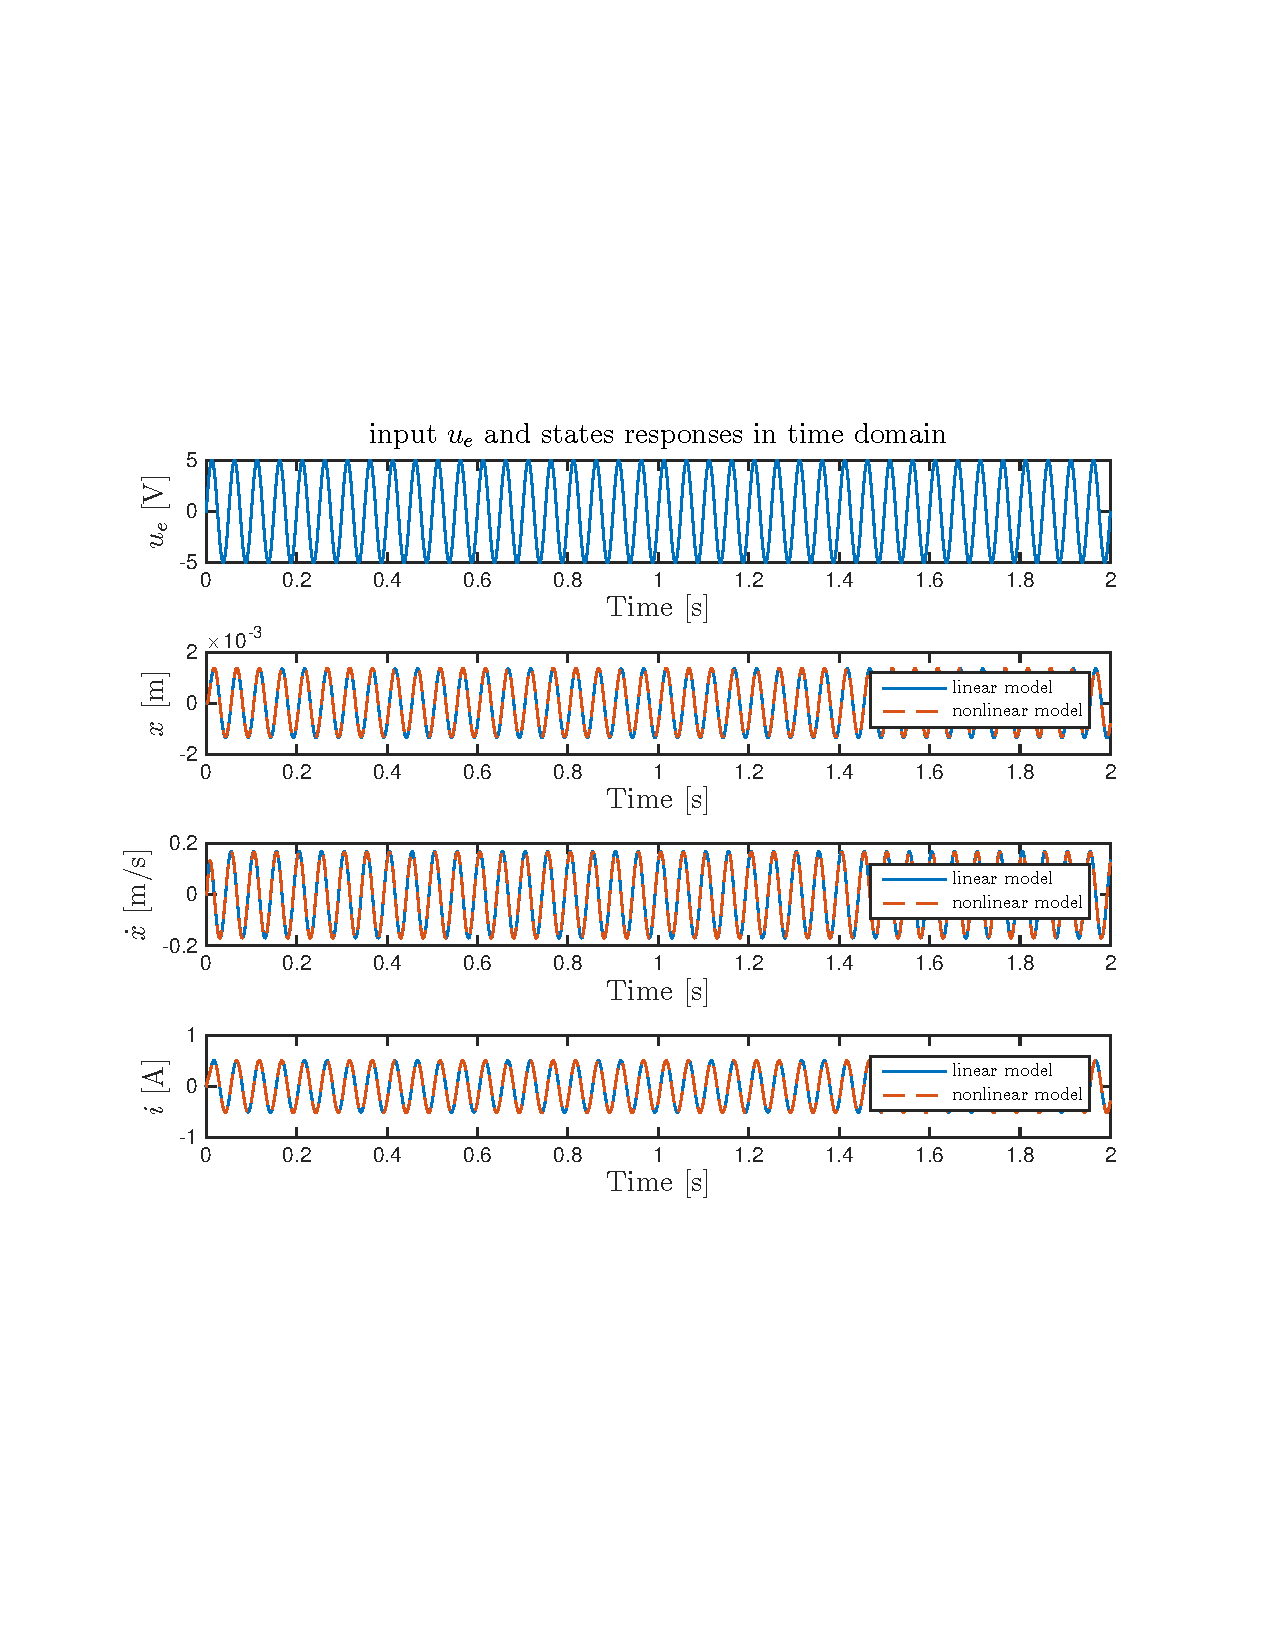
\includegraphics[trim=2cm 7cm 2cm 7cm, clip=true, totalheight=0.35\textheight, angle=0]{figures/p9time.pdf}
\caption{$u_e$ and states reponse to $u_e$ in time domain}
\label{fig:responseLMt}
\end{figure}
\begin{figure}[H]
 \centering 
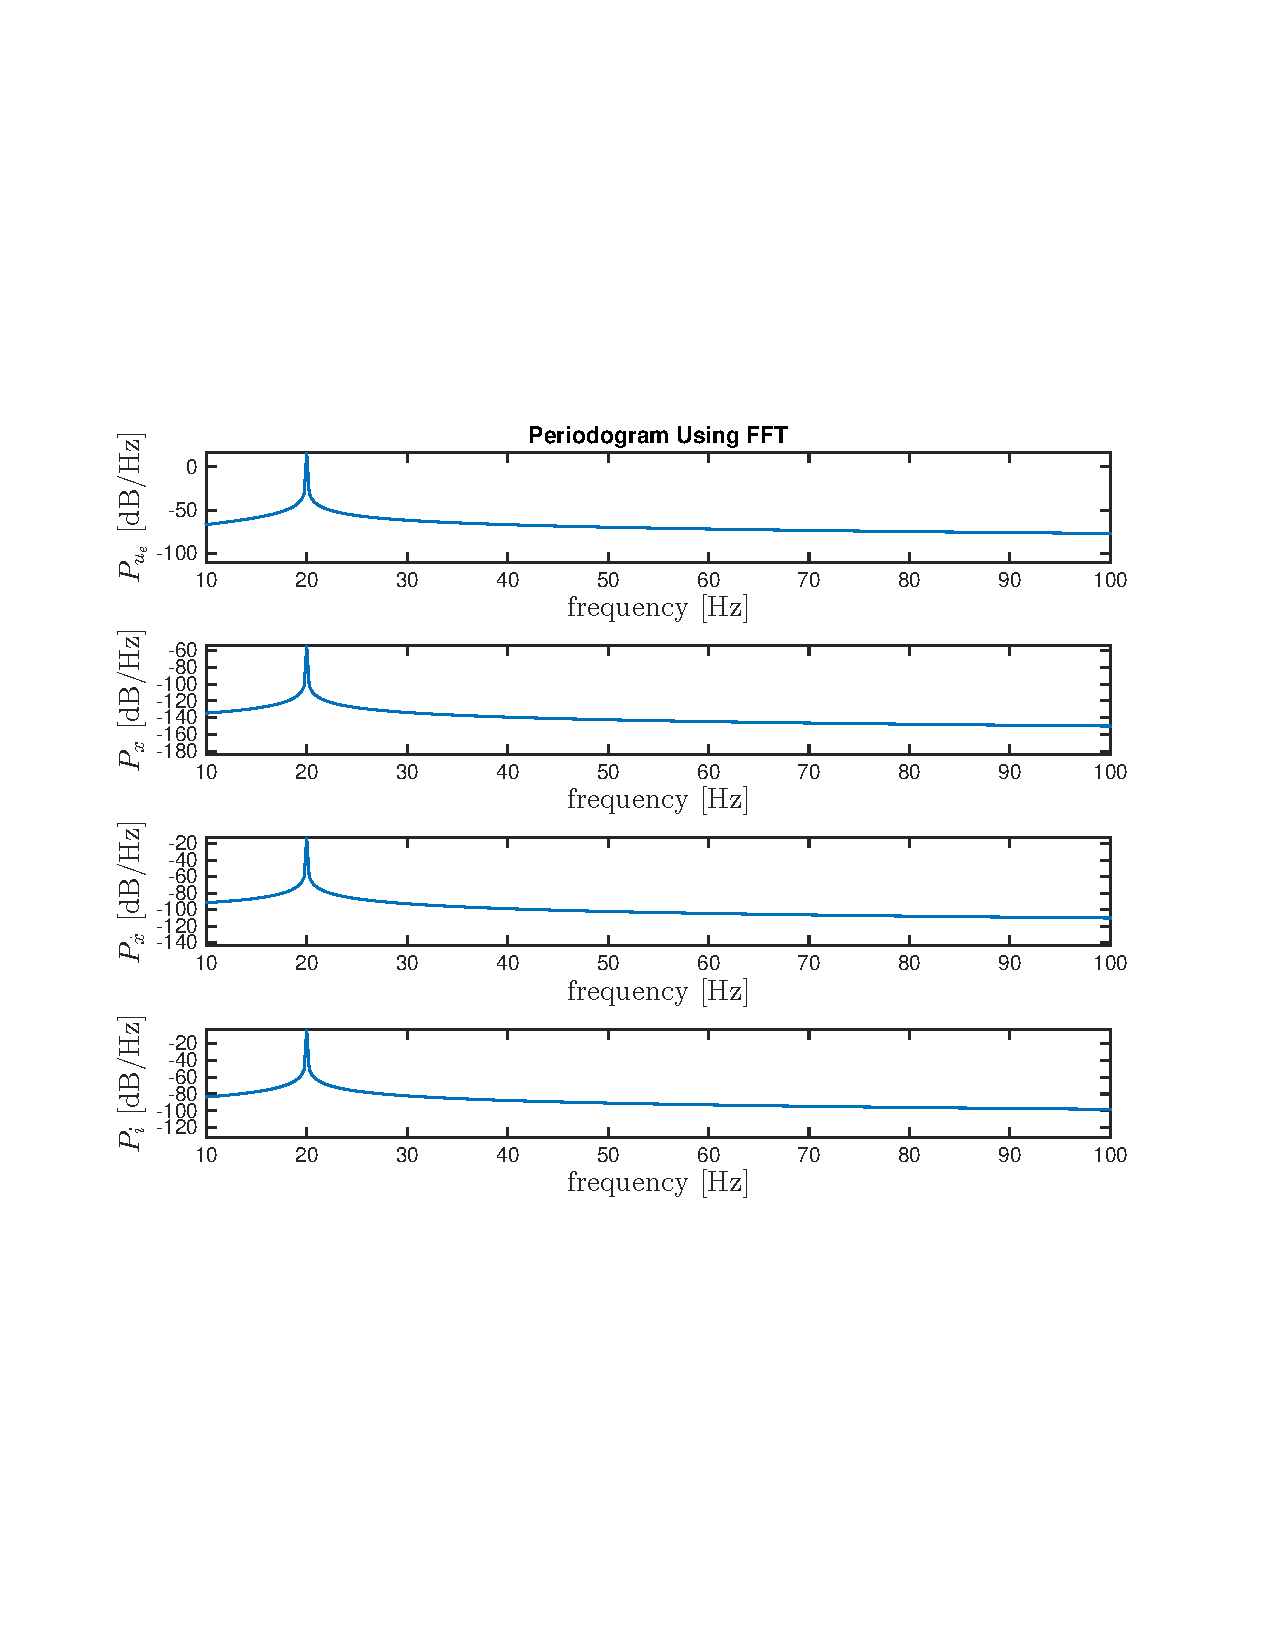
\includegraphics[trim=2cm 7cm 2cm 7cm, clip=true, totalheight=0.35\textheight, angle=0]{figures/p9freq.pdf}
\caption{PSD of $u_e$ and states}
\label{fig:responseLMf}
\end{figure}

First, comparing the response to the input $u_e$ from the nonlinear model with the linear model in the time domain (figure \ref{fig:NLMt}), the states response is almost exactly the same, but comparing the PSD of the states response (figure \ref{fig:NLMf} and figure \ref{fig:responseLMf}), we can see that the states response is not the same. Indeed, the linearised system is not affected by the harmonic distortion, there is only one frequency present in the states response, the one of 20$Hz$ (which has the same magnitude).
This result was expected because the nonlinear distortion only affects non-linear systems. Moreover, we have linearised the system with an input $u_e=0$ which means that we have a linearised system without harmonic, and then, we used a new input $u_e$ with a frequency $f_c=20Hz$, which means we only obtain a state response with an harmonic of a frequency of $f_c$.





